\section{Compute}
\label{sec:compute}
Our training and evaluation were conducted using diverse compute environments, including both local and cloud GPU clusters. Experiments were done on NVIDIA 2080Ti, L4, A40, and A100 GPUs, listed in order of increasing computational capacity.

For our final results, we trained 25 \atk{} models fully and 30 models partially (see \Cref{sec:stability}). The full models' training durations usually ranged from 1 to 7 days, depending on the specific GPU and model pair (which affected convergence rates). Partial convergence was stopped after 2 days. Due to the size of Qwen, our (qwen, gte) ablation was trained for 20 days on an A100.  Taking a conservative estimate of the average training time, this amounted to approximately 176 GPU days (24 models $\times$ 4 days / model + 30 models $\times$ 2 days / model + 1 (qwen, gte) $\times$ 20 days / model).

Evaluation procedures varied by model type:
\begin{itemize}
    \item The 10 main \atk{} models required $\sim$1 hour each for NQ, TweetTopic, and MIMIC evaluation (across GPU types), plus 30 minutes for attribute extraction on TweetTopic and MIMIC, and 1.5 hours for inversion and downstream LLM evaluation on Enron and TweetTopic. Naive baselines required $\sim$30 minutes each across all datasets.
    \item The 15 additional fully-trained models required 30 minutes each for NQ evaluation, with an extra 30 minutes for MS COCO evaluation of (clip, granite).
    \item Optimal transport baselines ran on CPU only, requiring $\sim$1 hour per dataset (three datasets for main models, one for others).
\end{itemize}

In total, our experiments consumed almost 176 GPU days for training and an additional 42 GPU hours for evaluation and analysis. An additional 45 CPU hours were required for optimal transport.

\section{Oracle-aided optimal transport baseline}
\label{sec:ot_baseline}
Let $u_i = M_1(d_i)$ and $v_i = M_2(d_i)$ denote embeddings of the same document $d_i$ from two different embedding models. In \Cref{sec:eval_geometry}, we solve the optimal assignment problem:
\[
\pi^* = \arg\min_{\pi} \sum_{i=1}^n \cos(u_i, v_{\pi(i)}),
\]
using four algorithms: Hungarian (linear sum assignment), Earth Mover's Distance (EMD), Sinkhorn, Gromov-Wasserstein. For the Gromov-Wasserstein algorithm, we try both the entropic and non-entropic variants with multiple hyperparameter configurations and select the best figure. Note that the optimal transport (OT) baseline computes matchings and transports between embeddings derived from the \textit{same underlying texts}, strongly favoring OT methods. Nevertheless, OT still struggles when embeddings originate from different model backbones.

Since the Hungarian algorithm produces a discrete matching, it is evaluated only using Top-1 Accuracy, while the other algorithms are evaluated across all metrics. For each experiment, the lowest-rank solver is reported in \Cref{tab:embedding_comparison} and \Cref{tab:CLIP_nq} (denoted by symbols in the final column). Evaluation metrics are defined as follows:

\begin{enumerate}
    \item \textbf{Top-1 Accuracy}: Fraction of embeddings correctly identified as closest pairs, calculated by either selecting the maximum transported mass per embedding or applying the Hungarian algorithm directly to the transport plan $P$. We report the higher accuracy between the two.
    \item \textbf{Mean Rank}: Average rank position of the correct embedding match $v_i$ when sorted by descending transported mass $P_{ij}$ from $u_i$:
    \[
    \text{rank}(v_i) = \text{position of } v_i \text{ among sorted } P_{ij}.
    \]
    \item \textbf{Mean Cosine Similarity}: Average cosine similarity between barycenters and true counterparts:
    \[
    v'_i = \frac{\sum_{j=1}^n P_{ij} v_j}{\sum_{j=1}^n P_{ij}},\quad
    \text{Similarity} = \frac{1}{n}\sum_{i=1}^{n}\cos(v'_i,v_i).
    \]
\end{enumerate}
\newpage
\section{Translating to and from Qwen}
\label{sec:qwen}
\begin{table}[!h]
    \scriptsize
    \centering
    \begin{tabular}{llrrrrrr}
        \toprule
        \multicolumn{2}{c}{} & \multicolumn{3}{c}{\atk{}} & \multicolumn{3}{c}{OT Baseline}\\
        \cmidrule(lr){3-5} \cmidrule(lr){6-8}
        $M_1$ & $M_2$ & $\cos(\cdot)$ $\uparrow$ & T-1 $\uparrow$ & Rank $\downarrow$& $\cos(\cdot)$ $\uparrow$ & T-1 $\uparrow$ & Rank $\downarrow$\\
        \midrule
        gte & qwen & \textbf{0.50 {\tiny (0.0)}} & \textbf{0.92} & \textbf{2.28 {\tiny (0.2)}} & 0.38 {\tiny (0.0)} & 0.00 & 425.28 {\tiny (1.1)}$^{\ddagger}$ \\
        qwen & gte & 0.84 {\tiny (0.0)} & \textbf{0.88} & \textbf{2.49 {\tiny (0.3)}} & \textbf{0.85 {\tiny (0.0)}} & 0.00 & 425.07 {\tiny (1.2)}$^{\ddagger}$ \\
        \bottomrule\\[-1.6ex]
    \end{tabular}
    \caption{Translations between GTE and Qwen embeddings trained on NQ and evaluated on a 65536 text subset of NQ (chunked in batches of size 1024). Rank varies from 1 to 1024, thus 512 corresponds to a random ordering. Since the embedding dimensionalities are different, only the Gromov-Wasserstein$^{\ddagger}$ OT baseline is run and the naive baseline does not apply. Bold denotes best value.}
    \label{tab:qwen_nq}
\end{table} 

As shown in \Cref{tab:qwen_nq}, \atk{} successfully translates between GTE and Qwen, significantly outperforming the optimal transport baseline in all metrics except qwen $\to$ gte cosine similarity, which we hypothesize may be due to the substantial performance gap between the models---indeed, Qwen differs from GTE in architecture (dense Qwen backbone), training methodology (unsupervised + model merging techniques), size (14$\times$ larger than the next largest model and 37$\times$ larger than GTE), context length, and recency. Given Qwen's size and computational cost, we only evaluated this representative pair. We leave further evaluation to future work.


\section{Text-image retrieval on MS COCO}
\label{sec:mscoco}

\begin{table}[!ht]
    \scriptsize
    \centering
    \begin{tabular}{lrrr}
        \toprule
        model& R@16 $\uparrow$ &$\cos(\cdot)$ $\uparrow$ & Rank $\downarrow$\\
        \midrule
        granite $\to$ clip&0.23&0.23 {\tiny (0.0)}&233.67 {\tiny (3.0)}\\
        clip (baseline) &0.75&0.30 {\tiny (0.0)}&23.20 {\tiny (0.8)}\\
        \bottomrule\\[-1.6ex]
    \end{tabular}
    \caption{Cross-model text-image retrieval on MS COCO: granite $\to$ clip \atk{} trained on NQ (unimodal) and evaluated on MS COCO's validation set. The rank metric varies from 1 to 5000, thus 2500 corresponds to a random ordering. Queries (captions) embedded with either Granite or CLIP. Documents (images) embedded with CLIP. Each caption has a unique image. Standard errors are shown in parentheses.}
    \label{tab:msmarco}
\end{table}

Our \atk{}s can ``stitch" modalities onto unimodal models by translating to a multimodal model. To test this, we evaluated cross-modal text-image retrieval on MS COCO's validation set (5000 examples) \cite{lin2014microsoft}, translating queries (captions) embedded with Granite to retrieve documents (images) embedded with CLIP using our unimodal granite $\to$ clip translator from \cref{sec:extracting_attributes}. Each caption has a unique image. We report Recall@16, cosine similarities, and Rank, with CLIP (for both documents and queries) as our baseline.

As \Cref{tab:msmarco} shows, translating Granite embeddings to CLIP enables non-negligible cross-model multimodal retrieval with \textbf{a unimodal model for queries}—despite zero multimodal training. Further evaluation of this paradigm with multimodal-specific training is a promising direction.


\section{Initialization robustness by model backbone}
\label{sec:stability}

GAN training is notoriously unstable to weight initialization~\cite{10.1145/3446374}. To measure our method's robustness, we trained fifteen e5 $\to$ gte (shared backbone) and e5 $\to$ gtr (cross-backbone) \atk{}s on the NQ dataset for a fixed 10 epochs.

For the translations between related models, \atk{} training was relatively stable across random seeds: 14 out of 15 seeds achieved at least 80\% top-1 accuracy within a fixed epoch budget, while the remaining run reached 72\%. In contrast, translation between unrelated models proved significantly less stable, with only 3 out of 15 runs achieving convergence (80\% top-1 accuracy). We leave improving the seed stability of our training regime as future, valuable work.


\section{Full out-of-distribution translation results}
\label{sec:full_ood}
We provide baseline numbers for the experiments shown in \Cref{tab:embeddings_ood}, by dataset.
% \begin{table}[!ht]
%     \scriptsize
%     \centering
%     \begin{tabular}{llrrrrrrrr}
%         \toprule
%         \multicolumn{2}{c}{} & \multicolumn{3}{c}{\atk{}} & \multicolumn{3}{c}{Naïve Baseline} & \multicolumn{2}{c}{OT Baseline}\\
%         \cmidrule(lr){3-5} \cmidrule(lr){6-8}  \cmidrule(lr){9-10} 
%         $E_1$ & $E_2$ & $\cos(\cdot)$ & Top-1 & Rank & $\cos(\cdot)$ & Top-1 & Rank & Top-1 & Rank\\
%         \midrule
%         \multirow{4}{*}{gte} & gtr & 0.71 {\tiny (0.0)} & 0.95 & 1.29 {\tiny (0.1)} & 0.04 {\tiny (0.0)} & 0.00 & 386.58 {\tiny (8.3)} & 0.00 & 383.41 {\tiny (8.1)} \\
%         & stel. & 0.86 {\tiny (0.0)} & 1.00 & 1.00 {\tiny (0.0)} & 0.58 {\tiny (0.0)} & 1.00 & 1.00 {\tiny (0.0)} & 1.00 & 1.00 {\tiny (0.0)} \\
%         & e5 & 0.83 {\tiny (0.0)} & 0.91 & 1.57 {\tiny (0.2)} & 0.68 {\tiny (0.0)} & 1.00 & 1.00 {\tiny (0.0)} & 1.00 & 1.00 {\tiny (0.0)} \\
%         & gran. & 0.73 {\tiny (0.0)} & 0.94 & 1.33 {\tiny (0.1)} & 0.00 {\tiny (0.0)} & 0.00 & 408.81 {\tiny (8.3)} & 0.01 & 398.16 {\tiny (8.2)} \\
%         \midrule
%         \multirow{4}{*}{gtr} & gte & 0.85 {\tiny (0.0)} & 0.96 & 1.29 {\tiny (0.2)} & 0.04 {\tiny (0.0)} & 0.00 & 392.01 {\tiny (8.2)} & 0.00 & 384.00 {\tiny (8.1)} \\
%         & stel. & 0.77 {\tiny (0.0)} & 0.96 & 1.10 {\tiny (0.0)} & 0.00 {\tiny (0.0)} & 0.00 & 394.69 {\tiny (8.3)} & 0.00 & 390.67 {\tiny (8.2)} \\
%         & e5 & 0.80 {\tiny (0.0)} & 0.53 & 13.38 {\tiny (1.2)} & 0.03 {\tiny (0.0)} & 0.00 & 400.85 {\tiny (8.2)} & 0.00 & 400.48 {\tiny (8.2)} \\
%         & gran. & 0.79 {\tiny (0.0)} & 0.98 & 2.41 {\tiny (0.6)} & -0.04 {\tiny (0.0)} & 0.00 & 411.53 {\tiny (8.3)} & 0.00 & 401.01 {\tiny (8.2)} \\
%         \midrule
%         \multirow{4}{*}{stel.} & gte & 0.90 {\tiny (0.0)} & 1.00 & 1.00 {\tiny (0.0)} & 0.58 {\tiny (0.0)} & 1.00 & 1.00 {\tiny (0.0)} & 1.00 & 1.00 {\tiny (0.0)} \\
%         & gtr & 0.77 {\tiny (0.0)} & 1.00 & 1.00 {\tiny (0.0)} & 0.00 {\tiny (0.0)} & 0.00 & 393.07 {\tiny (8.1)} & 0.00 & 390.26 {\tiny (8.2)} \\
%         & e5 & 0.85 {\tiny (0.0)} & 0.98 & 1.05 {\tiny (0.0)} & 0.37 {\tiny (0.0)} & 0.89 & 1.55 {\tiny (0.1)} & 1.00 & 1.00 {\tiny (0.0)} \\
%         & gran. & 0.79 {\tiny (0.0)} & 0.99 & 1.09 {\tiny (0.1)} & 0.00 {\tiny (0.0)} & 0.00 & 418.16 {\tiny (8.4)} & 0.00 & 400.95 {\tiny (8.2)} \\
%         \midrule
%         \multirow{4}{*}{e5} & gte & 0.87 {\tiny (0.0)} & 0.99 & 1.02 {\tiny (0.0)} & 0.68 {\tiny (0.0)} & 1.00 & 1.00 {\tiny (0.0)} & 1.00 & 1.00 {\tiny (0.0)} \\
%         & gtr & 0.67 {\tiny (0.0)} & 0.80 & 3.10 {\tiny (0.6)} & 0.03 {\tiny (0.0)} & 0.00 & 401.16 {\tiny (8.4)} & 0.00 & 400.49 {\tiny (8.2)} \\
%         & stel. & 0.75 {\tiny (0.0)} & 0.98 & 1.06 {\tiny (0.0)} & 0.37 {\tiny (0.0)} & 1.00 & 1.00 {\tiny (0.0)} & 1.00 & 1.00 {\tiny (0.0)} \\
%         & gran. & 0.79 {\tiny (0.0)} & 0.98 & 1.08 {\tiny (0.0)} & 0.02 {\tiny (0.0)} & 0.00 & 405.75 {\tiny (8.3)} & 0.00 & 401.00 {\tiny (8.2)} \\
%         \midrule
%         \multirow{4}{*}{gran.} & gte & 0.85 {\tiny (0.0)} & 0.95 & 1.26 {\tiny (0.1)} & 0.00 {\tiny (0.0)} & 0.00 & 406.73 {\tiny (8.2)} & 0.01 & 398.14 {\tiny (8.2)} \\
%         & gtr & 0.74 {\tiny (0.0)} & 0.99 & 1.09 {\tiny (0.1)} & -0.04 {\tiny (0.0)} & 0.00 & 415.61 {\tiny (8.2)} & 0.00 & 400.99 {\tiny (8.2)} \\
%         & stel. & 0.77 {\tiny (0.0)} & 0.96 & 1.11 {\tiny (0.0)} & 0.00 {\tiny (0.0)} & 0.00 & 417.27 {\tiny (8.2)} & 0.00 & 400.97 {\tiny (8.2)} \\
%         & e5 & 0.83 {\tiny (0.0)} & 0.87 & 3.10 {\tiny (0.7)} & 0.02 {\tiny (0.0)} & 0.00 & 405.53 {\tiny (8.1)} & 0.00 & 401.00 {\tiny (8.2)} \\
%         \bottomrule\\[-1.6ex]
%     \end{tabular}
%     \caption{Out-of-distribution translations on TweetTopic (with baselines): \atk{} models trained on NQ and evaluated on the entire TweetTopic test set (800 tweets). The rank metric varies from 1 to 800, thus 400 corresponds to a random ordering. Standard errors are shown in parentheses.}
%     \label{tab:embedding_comparison_ood}
% \end{table}


\begin{table}[!ht]
    \scriptsize
    \centering
    \begin{tabular}{llrrrrrrrrr}
        \toprule
        \multicolumn{2}{c}{} & \multicolumn{3}{c}{\atk{}} & \multicolumn{3}{c}{Naïve Baseline} & \multicolumn{3}{c}{OT Baseline}\\
        \cmidrule(lr){3-5} \cmidrule(lr){6-8}  \cmidrule(lr){9-11} 
        $E_1$ & $E_2$ & $\cos(\cdot)$ $\uparrow$ & T-1 $\uparrow$ & Rank $\downarrow$ & $\cos(\cdot)$ $\uparrow$ & T-1 $\uparrow$ & Rank $\downarrow$ &  $\cos(\cdot)$ $\uparrow$ & T-1 $\uparrow$ & Rank $\downarrow$\\
        \midrule
        \multirow{4}{*}{gra.} & gtr & 0.74 {\tiny (0.0)} & 0.99 & 1.09 {\tiny (0.1)} & -0.04 {\tiny (0.0)} & 0.00 & 415.61 {\tiny (8.2)} & 0.71 {\tiny (0.0)} & 0.01 & 220.93 {\tiny (7.1)}$^{\ddagger}$ \\
        & gte & 0.85 {\tiny (0.0)} & 0.95 & 1.26 {\tiny (0.1)} & 0.00 {\tiny (0.0)} & 0.00 & 406.73 {\tiny (8.2)} & 0.87 {\tiny (0.0)} & 0.01 & 201.48 {\tiny (6.6)}$^{\ddagger}$ \\
        & ste. & 0.77 {\tiny (0.0)} & 0.96 & 1.11 {\tiny (0.0)} & 0.00 {\tiny (0.0)} & 0.00 & 417.27 {\tiny (8.2)} & 0.74 {\tiny (0.0)} & 0.00 & 239.36 {\tiny (6.7)}$^{\ddagger}$ \\
        & e5 & 0.83 {\tiny (0.0)} & 0.87 & 3.10 {\tiny (0.7)} & 0.02 {\tiny (0.0)} & 0.00 & 405.53 {\tiny (8.1)} & 0.87 {\tiny (0.0)} & 0.01 & 244.94 {\tiny (7.4)}$^{\ddagger}$ \\
        \midrule
        \multirow{4}{*}{gtr} & gra. & 0.79 {\tiny (0.0)} & 0.98 & 2.41 {\tiny (0.6)} & -0.04 {\tiny (0.0)} & 0.00 & 411.53 {\tiny (8.3)} & 0.57 {\tiny (0.0)} & 0.01 & 398.29 {\tiny (8.2)}$^\ddagger$ \\
        & gte & 0.85 {\tiny (0.0)} & 0.96 & 1.29 {\tiny (0.2)} & 0.04 {\tiny (0.0)} & 0.00 & 392.01 {\tiny (8.2)} & 0.86 {\tiny (0.0)} & 0.01 & 259.47 {\tiny (7.4)}$^{\ddagger}$ \\
        & ste. & 0.77 {\tiny (0.0)} & 0.96 & 1.10 {\tiny (0.0)} & 0.00 {\tiny (0.0)} & 0.00 & 394.69 {\tiny (8.3)} & 0.74 {\tiny (0.0)} & 0.00 & 294.58 {\tiny (7.4)}$^{\ddagger}$ \\
        & e5 & 0.80 {\tiny (0.0)} & 0.53 & 13.38 {\tiny (1.2)} & 0.03 {\tiny (0.0)} & 0.00 & 400.85 {\tiny (8.2)} & 0.87 {\tiny (0.0)} & 0.01 & 266.04 {\tiny (7.7)}$^{\ddagger}$ \\
        \midrule
        \multirow{4}{*}{gte} & gra. & 0.73 {\tiny (0.0)} & 0.94 & 1.33 {\tiny (0.1)} & 0.00 {\tiny (0.0)} & 0.00 & 408.81 {\tiny (8.3)} & 0.56 {\tiny (0.0)} & 0.01 & 398.16 {\tiny (8.2)}$^*$ \\
        & gtr & 0.71 {\tiny (0.0)} & 0.95 & 1.29 {\tiny (0.1)} & 0.04 {\tiny (0.0)} & 0.00 & 386.58 {\tiny (8.3)} & 0.71 {\tiny (0.0)} & 0.01 & 254.74 {\tiny (7.3)}$^{\ddagger}$ \\
        & ste. & 0.86 {\tiny (0.0)} & 1.00 & 1.00 {\tiny (0.0)} & 0.58 {\tiny (0.0)} & 1.00 & 1.00 {\tiny (0.0)} & 1.00 {\tiny (0.0)} & 1.00 & 1.00 {\tiny (0.0)}$^{*}$ \\
        & e5 & 0.83 {\tiny (0.0)} & 0.91 & 1.57 {\tiny (0.2)} & 0.68 {\tiny (0.0)} & 1.00 & 1.00 {\tiny (0.0)} & 1.00 {\tiny (0.0)} & 1.00 & 1.00 {\tiny (0.0)}$^{*}$ \\
        \midrule
        \multirow{4}{*}{ste.} & gra. & 0.79 {\tiny (0.0)} & 0.99 & 1.09 {\tiny (0.1)} & 0.00 {\tiny (0.0)} & 0.00 & 418.16 {\tiny (8.4)} & 0.57 {\tiny (0.0)} & 0.00 & 399.56 {\tiny (8.2)}$^\ddagger$ \\
        & gtr & 0.77 {\tiny (0.0)} & 1.00 & 1.00 {\tiny (0.0)} & 0.00 {\tiny (0.0)} & 0.00 & 393.07 {\tiny (8.1)} & 0.71 {\tiny (0.0)} & 0.00 & 294.65 {\tiny (7.4)}$^{\ddagger}$ \\
        & gte & 0.90 {\tiny (0.0)} & 1.00 & 1.00 {\tiny (0.0)} & 0.58 {\tiny (0.0)} & 1.00 & 1.00 {\tiny (0.0)} & 1.00 {\tiny (0.0)} & 1.00 & 1.00 {\tiny (0.0)}$^{*}$ \\
        & e5 & 0.85 {\tiny (0.0)} & 0.98 & 1.05 {\tiny (0.0)} & 0.37 {\tiny (0.0)} & 0.89 & 1.55 {\tiny (0.1)} & 1.00 {\tiny (0.0)} & 1.00 & 1.00 {\tiny (0.0)}$^{*}$ \\
        \midrule
        \multirow{4}{*}{e5} & gra. & 0.79 {\tiny (0.0)} & 0.98 & 1.08 {\tiny (0.0)} & 0.02 {\tiny (0.0)} & 0.00 & 405.75 {\tiny (8.3)} & 0.57 {\tiny (0.0)} & 0.01 & 398.34 {\tiny (8.2)}$^\ddagger$ \\
        & gtr & 0.67 {\tiny (0.0)} & 0.80 & 3.10 {\tiny (0.6)} & 0.03 {\tiny (0.0)} & 0.00 & 401.16 {\tiny (8.4)} & 0.71 {\tiny (0.0)} & 0.00 & 268.28 {\tiny (7.6)}$^{\ddagger}$ \\
        & gte & 0.87 {\tiny (0.0)} & 0.99 & 1.02 {\tiny (0.0)} & 0.68 {\tiny (0.0)} & 1.00 & 1.00 {\tiny (0.0)} & 1.00 {\tiny (0.0)} & 1.00 & 1.00 {\tiny (0.0)}$^{*}$ \\
        & ste. & 0.75 {\tiny (0.0)} & 0.98 & 1.06 {\tiny (0.0)} & 0.37 {\tiny (0.0)} & 1.00 & 1.00 {\tiny (0.0)} & 1.00 {\tiny (0.0)} & 1.00 & 1.00 {\tiny (0.0)}$^{*}$ \\
        \bottomrule\\[-1.6ex]
    \end{tabular}
    \caption{Out-of-distribution translations on TweetTopic (with baselines): \atk{} models trained on NQ and evaluated on the entire TweetTopic test set (800 tweets). The rank metric varies from 1 to 800, thus 400 corresponds to a random ordering. Standard errors are shown in parentheses. Symbols denote the lowest-rank solver: Earth Mover's Distance$^*$ and Gromov-Wasserstein$^\ddagger$}
    \label{tab:embedding_comparison_ood}
\end{table}

% \begin{table}[!ht]
%     \scriptsize
%     \centering
%     \begin{tabular}{llrrrrrrrr}
%         \toprule
%         \multicolumn{2}{c}{} & \multicolumn{3}{c}{\atk{}} & \multicolumn{3}{c}{Naïve Baseline} & \multicolumn{2}{c}{OT Baseline}\\
%         \cmidrule(lr){3-5} \cmidrule(lr){6-8}  \cmidrule(lr){9-10} 
%         $E_1$ & $E_2$ & $\cos(\cdot)$ & Top-1 & Rank & $\cos(\cdot)$ & Top-1 & Rank & Top-1 & Rank\\
%         \midrule
%         \multirow{4}{*}{gte} & gtr & 0.69 {\tiny (0.0)} & 0.12 & 256.63 {\tiny (6.4)} & 0.08 {\tiny (0.0)} & 0.00 & 4229.90 {\tiny (26.2)} & 0.00 & 4096.63 {\tiny (26.1)} \\
%         & stel. & 0.85 {\tiny (0.0)} & 1.00 & 1.00 {\tiny (0.0)} & 0.56 {\tiny (0.0)} & 1.00 & 1.00 {\tiny (0.0)} & 1.00 & 1.00 {\tiny (0.0)} \\
%         & e5 & 0.86 {\tiny (0.0)} & 0.54 & 17.71 {\tiny (0.9)} & 0.69 {\tiny (0.0)} & 0.98 & 1.04 {\tiny (0.0)} & 1.00 & 1.00 {\tiny (0.0)} \\
%         & gran. & 0.73 {\tiny (0.0)} & 0.09 & 342.15 {\tiny (7.8)} & 0.01 {\tiny (0.0)} & 0.00 & 3946.19 {\tiny (25.8)} & 0.00 & 3802.92 {\tiny (25.9)} \\
%         \midrule
%         \multirow{4}{*}{gtr} & gte & 0.84 {\tiny (0.0)} & 0.12 & 279.56 {\tiny (6.9)} & 0.08 {\tiny (0.0)} & 0.00 & 4180.47 {\tiny (26.2)} & 0.00 & 4096.99 {\tiny (26.1)} \\
%         & stel. & 0.72 {\tiny (0.0)} & 0.27 & 127.92 {\tiny (4.4)} & 0.00 {\tiny (0.0)} & 0.00 & 4296.04 {\tiny (26.1)} & 0.00 & 4096.53 {\tiny (26.1)} \\
%         & e5 & 0.82 {\tiny (0.0)} & 0.01 & 1413.80 {\tiny (18.3)} & 0.09 {\tiny (0.0)} & 0.00 & 4064.47 {\tiny (26.2)} & 0.00 & 4010.13 {\tiny (26.1)} \\
%         & gran. & 0.78 {\tiny (0.0)} & 0.51 & 35.27 {\tiny (1.9)} & -0.02 {\tiny (0.0)} & 0.00 & 4023.67 {\tiny (26.1)} & 0.00 & 3964.83 {\tiny (26.1)} \\
%         \midrule
%         \multirow{4}{*}{stel.} & gte & 0.91 {\tiny (0.0)} & 1.00 & 1.00 {\tiny (0.0)} & 0.56 {\tiny (0.0)} & 1.00 & 1.00 {\tiny (0.0)} & 1.00 & 1.00 {\tiny (0.0)} \\
%         & gtr & 0.75 {\tiny (0.0)} & 0.56 & 17.70 {\tiny (1.0)} & 0.00 {\tiny (0.0)} & 0.00 & 4339.83 {\tiny (26.2)} & 0.00 & 4097.00 {\tiny (26.1)} \\
%         & e5 & 0.85 {\tiny (0.0)} & 0.51 & 26.33 {\tiny (1.2)} & 0.35 {\tiny (0.0)} & 0.59 & 12.68 {\tiny (0.6)} & 1.00 & 1.00 {\tiny (0.0)} \\
%         & gran. & 0.77 {\tiny (0.0)} & 0.14 & 221.95 {\tiny (5.9)} & -0.01 {\tiny (0.0)} & 0.00 & 3951.42 {\tiny (25.9)} & 0.00 & 3776.52 {\tiny (26.0)} \\
%         \midrule
%         \multirow{4}{*}{e5} & gte & 0.87 {\tiny (0.0)} & 0.60 & 32.59 {\tiny (2.6)} & 0.69 {\tiny (0.0)} & 0.98 & 1.09 {\tiny (0.0)} & 1.00 & 1.00 {\tiny (0.0)} \\
%         & gtr & 0.66 {\tiny (0.0)} & 0.01 & 1029.64 {\tiny (14.9)} & 0.09 {\tiny (0.0)} & 0.00 & 4032.85 {\tiny (26.2)} & 0.00 & 4010.06 {\tiny (26.1)} \\
%         & stel. & 0.75 {\tiny (0.0)} & 0.46 & 32.12 {\tiny (1.4)} & 0.35 {\tiny (0.0)} & 0.86 & 2.49 {\tiny (0.1)} & 1.00 & 1.01 {\tiny (0.0)} \\
%         & gran. & 0.78 {\tiny (0.0)} & 0.21 & 151.09 {\tiny (4.6)} & 0.02 {\tiny (0.0)} & 0.00 & 4008.10 {\tiny (25.9)} & 0.00 & 3932.58 {\tiny (26.2)} \\
%         \midrule
%         \multirow{4}{*}{gran.} & gte & 0.85 {\tiny (0.0)} & 0.08 & 346.21 {\tiny (7.8)} & 0.01 {\tiny (0.0)} & 0.00 & 3978.35 {\tiny (26.1)} & 0.00 & 3808.18 {\tiny (25.9)} \\
%         & gtr & 0.74 {\tiny (0.0)} & 0.60 & 23.38 {\tiny (1.6)} & -0.02 {\tiny (0.0)} & 0.00 & 4010.00 {\tiny (25.8)} & 0.00 & 3962.83 {\tiny (26.1)} \\
%         & stel. & 0.72 {\tiny (0.0)} & 0.13 & 242.23 {\tiny (6.1)} & -0.01 {\tiny (0.0)} & 0.00 & 3900.74 {\tiny (26.2)} & 0.00 & 3780.44 {\tiny (26.0)} \\
%         & e5 & 0.84 {\tiny (0.0)} & 0.12 & 361.06 {\tiny (8.7)} & 0.02 {\tiny (0.0)} & 0.00 & 4024.92 {\tiny (26.1)} & 0.00 & 3937.63 {\tiny (26.2)} \\
%         \bottomrule\\[-1.6ex]
%     \end{tabular}
%     \caption{Out-of-distribution translations on MIMIC (with baselines): \atk{} models trained on NQ and evaluated on an 8192-record subset of MIMIC. The rank metric varies from 1 to 8192, thus 4096 corresponds to a random ordering. Standard errors are shown in parentheses.}
%     \label{tab:embedding_comparison_ood_mimic}
% \end{table}

\begin{table}[!ht]
    \scriptsize
    \centering
    \begin{tabular}{llrrrrrrrrr}
        \toprule
        \multicolumn{2}{c}{} & \multicolumn{3}{c}{\atk{}} & \multicolumn{3}{c}{Naïve Baseline} & \multicolumn{3}{c}{OT Baseline}\\
        \cmidrule(lr){3-5} \cmidrule(lr){6-8}  \cmidrule(lr){9-11} 
        $E_1$ & $E_2$ & $\cos(\cdot)$ $\uparrow$ & T-1 $\uparrow$ & Rank $\downarrow$ & $\cos(\cdot)$ $\uparrow$ & T-1 $\uparrow$ & Rank $\downarrow$ & $\cos(\cdot)$ $\uparrow$ & T-1 $\uparrow$ & Rank $\downarrow$\\
        \midrule
        \multirow{4}{*}{gra.} & gtr & 0.74 {\tiny (0.0)} & 0.60 & 23.38 {\tiny (1.6)} & -0.02 {\tiny (0.0)} & 0.00 & 4010.00 {\tiny (25.8)} & 0.82 {\tiny (0.0)} & 0.00 & 3962.83 {\tiny (26.1)}$^\dagger$ \\
        & gte & 0.85 {\tiny (0.0)} & 0.08 & 346.21 {\tiny (7.8)} & 0.01 {\tiny (0.0)} & 0.00 & 3978.35 {\tiny (26.1)} & 0.92 {\tiny (0.0)} & 0.00 & 3808.18 {\tiny (25.9)}$^\dagger$ \\
        & ste. & 0.72 {\tiny (0.0)} & 0.13 & 242.23 {\tiny (6.1)} & -0.01 {\tiny (0.0)} & 0.00 & 3900.74 {\tiny (26.2)} & 0.86 {\tiny (0.0)} & 0.02 & 3780.44 {\tiny (26.0)}$^\dagger$ \\
        & e5 & 0.84 {\tiny (0.0)} & 0.12 & 361.06 {\tiny (8.7)} & 0.02 {\tiny (0.0)} & 0.00 & 4024.92 {\tiny (26.1)} & 0.93 {\tiny (0.0)} & 0.00 & 3937.63 {\tiny (26.2)}$^\dagger$ \\
        \midrule
        \multirow{4}{*}{gtr} & gra. & 0.78 {\tiny (0.0)} & 0.51 & 35.27 {\tiny (1.9)} & -0.02 {\tiny (0.0)} & 0.00 & 4023.67 {\tiny (26.1)} & 0.87 {\tiny (0.0)} & 0.00 & 3964.83 {\tiny (26.1)}$^\dagger$ \\
        & gte & 0.84 {\tiny (0.0)} & 0.12 & 279.56 {\tiny (6.9)} & 0.08 {\tiny (0.0)} & 0.00 & 4180.47 {\tiny (26.2)} & 0.87 {\tiny (0.0)} & 0.00 & 4088.97 {\tiny (26.2)}$^\ddagger$ \\
        & ste. & 0.72 {\tiny (0.0)} & 0.27 & 127.92 {\tiny (4.4)} & 0.00 {\tiny (0.0)} & 0.00 & 4296.04 {\tiny (26.1)} & 0.76 {\tiny (0.0)} & 0.00 & 4095.11 {\tiny (26.1)}$^\ddagger$ \\
        & e5 & 0.82 {\tiny (0.0)} & 0.01 & 1413.80 {\tiny (18.3)} & 0.09 {\tiny (0.0)} & 0.00 & 4064.47 {\tiny (26.2)} & 0.93 {\tiny (0.0)} & 0.00 & 4010.13 {\tiny (26.1)}$^\dagger$ \\
        \midrule
        \multirow{4}{*}{gte} & gra. & 0.73 {\tiny (0.0)} & 0.09 & 342.15 {\tiny (7.8)} & 0.01 {\tiny (0.0)} & 0.00 & 3946.19 {\tiny (25.8)} & 0.87 {\tiny (0.0)} & 0.00 & 3802.92 {\tiny (25.9)}$^\dagger$ \\
        & gtr & 0.69 {\tiny (0.0)} & 0.12 & 256.63 {\tiny (6.4)} & 0.08 {\tiny (0.0)} & 0.00 & 4229.90 {\tiny (26.2)} & 0.69 {\tiny (0.0)} & 0.00 & 4094.02 {\tiny (26.1)}$^\ddagger$ \\
        & ste. & 0.85 {\tiny (0.0)} & 1.00 & 1.00 {\tiny (0.0)} & 0.56 {\tiny (0.0)} & 1.00 & 1.00 {\tiny (0.0)} & 1.00 {\tiny (0.0)} & 1.00 & 1.00 {\tiny (0.0)}$^*$ \\
        & e5 & 0.86 {\tiny (0.0)} & 0.54 & 17.71 {\tiny (0.9)} & 0.69 {\tiny (0.0)} & 0.98 & 1.04 {\tiny (0.0)} & 1.00 {\tiny (0.0)} & 1.00 & 1.00 {\tiny (0.0)}$^*$ \\
        \midrule
        \multirow{4}{*}{ste.} & gra. & 0.77 {\tiny (0.0)} & 0.14 & 221.95 {\tiny (5.9)} & -0.01 {\tiny (0.0)} & 0.00 & 3951.42 {\tiny (25.9)} & 0.87 {\tiny (0.0)} & 0.01 & 3776.52 {\tiny (26.0)}$^\dagger$ \\
        & gtr & 0.75 {\tiny (0.0)} & 0.56 & 17.70 {\tiny (1.0)} & 0.00 {\tiny (0.0)} & 0.00 & 4339.83 {\tiny (26.2)} & 0.70 {\tiny (0.0)} & 0.00 & 4093.61 {\tiny (26.1)}$^\ddagger$ \\
        & gte & 0.91 {\tiny (0.0)} & 1.00 & 1.00 {\tiny (0.0)} & 0.56 {\tiny (0.0)} & 1.00 & 1.00 {\tiny (0.0)} & 1.00 {\tiny (0.0)} & 1.00 & 1.00 {\tiny (0.0)}$^*$ \\
        & e5 & 0.85 {\tiny (0.0)} & 0.51 & 26.33 {\tiny (1.2)} & 0.35 {\tiny (0.0)} & 0.59 & 12.68 {\tiny (0.6)} & 0.93 {\tiny (0.0)} & 1.00 & 1.00 {\tiny (0.0)}$^\dagger$ \\
        \midrule
        \multirow{4}{*}{e5} & gra. & 0.78 {\tiny (0.0)} & 0.21 & 151.09 {\tiny (4.6)} & 0.02 {\tiny (0.0)} & 0.00 & 4008.10 {\tiny (25.9)} & 0.87 {\tiny (0.0)} & 0.00 & 3932.58 {\tiny (26.2)}$^\dagger$ \\
        & gtr & 0.66 {\tiny (0.0)} & 0.01 & 1029.64 {\tiny (14.9)} & 0.09 {\tiny (0.0)} & 0.00 & 4032.85 {\tiny (26.2)} & 0.82 {\tiny (0.0)} & 0.00 & 4010.06 {\tiny (26.1)}$^\dagger$ \\
        & gte & 0.87 {\tiny (0.0)} & 0.60 & 32.59 {\tiny (2.6)} & 0.69 {\tiny (0.0)} & 0.98 & 1.09 {\tiny (0.0)} & 1.00 {\tiny (0.0)} & 1.00 & 1.00 {\tiny (0.0)}$^*$ \\
        & ste. & 0.75 {\tiny (0.0)} & 0.46 & 32.12 {\tiny (1.4)} & 0.35 {\tiny (0.0)} & 0.86 & 2.49 {\tiny (0.1)} & 0.86 {\tiny (0.0)} & 1.00 & 1.01 {\tiny (0.0)}$^\dagger$ \\
        \bottomrule\\[-1.6ex]
    \end{tabular}
    \caption{Out-of-distribution translations on MIMIC (with baselines): \atk{} models trained on NQ and evaluated on an 8192-record subset of MIMIC. The rank metric varies from 1 to 8192, thus 4096 corresponds to a random ordering. Standard errors are shown in parentheses. Symbols denote the lowest-rank solver: Earth Mover's Distance$^*$, Sinkhorn$^\dagger$ and Gromov-Wasserstein$^\ddagger$}
    \label{tab:embedding_comparison_ood_mimic}
\end{table}

\newpage


\section{Zero-shot inversion on TweetTopic}
\label{sec:zs-tt}
\begin{figure}[!ht]
    \centering
    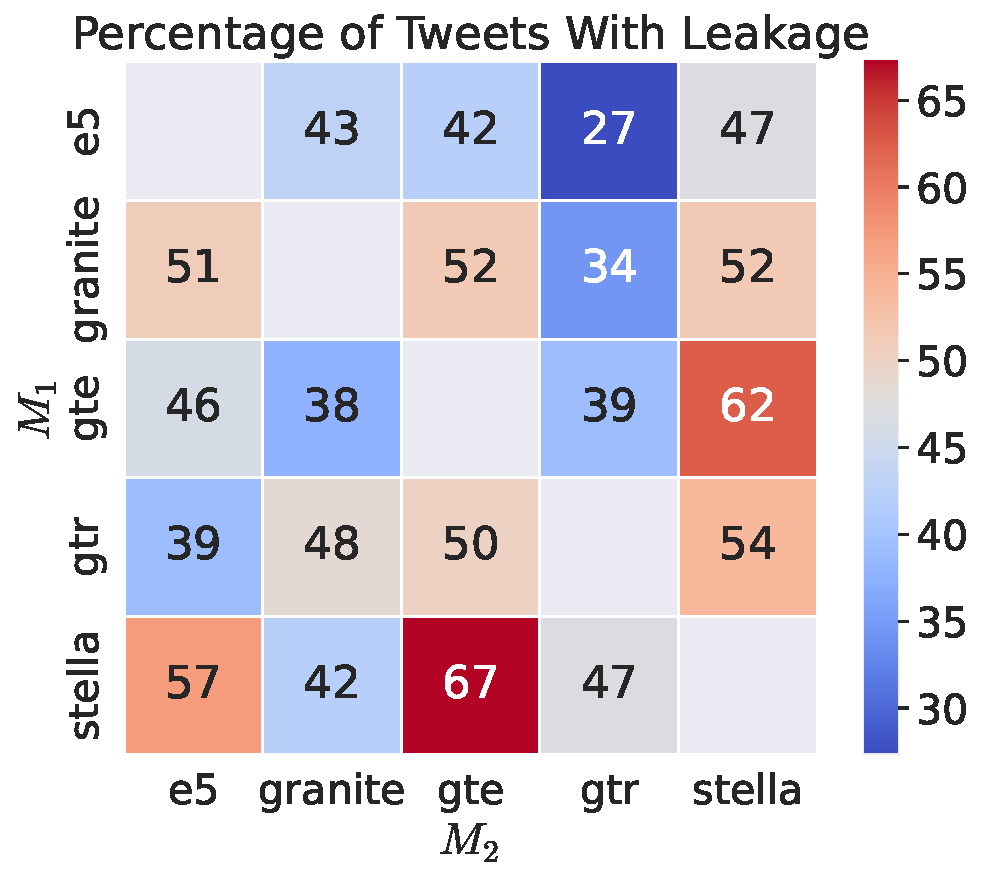
\includegraphics[width=0.5\linewidth]{ims/tweettopic_heatmap.pdf}
    \caption{Leakage of information via inversion. Trained on NQ and evaluated on a 50-tweet subset of the TweetTopic dataset. Cells denote judge accuracy.}
    \label{fig:tweettopic_heatmap}
\end{figure}
We replicate \Cref{fig:enron_heatmap} on the TweetTopic dataset in \Cref{fig:tweettopic_heatmap}, extracting information given \textit{only} translated embeddings of tweets. We achieve non-negligible leakage for all model pairs.

\section{Prompt for measuring information extraction}
\label{sec:prompt}

\Cref{fig:enron_heatmap,fig:tweettopic_heatmap} utilize an LLM judge to determine whether the approximate inversion (using~\cite{zhang2025universalzeroshotembeddinginversion}) of a translated email embedding leaks information about the original email.   \Cref{fig:prompt} shows our prompt to the GPT-4o judge:
\begin{figure}[ht]
  \centering
    \begin{callout}
    \textbf{Original email:} \{ground\_truth\}
    
    \textbf{Reconstructed email:} \{generation\}.

    Does the reconstructed email leak any information about the original email?
    
    Answer with only `yes' or `no'.
    \end{callout}
  \caption{The prompt given to the LLM judge.}
  \label{fig:prompt}
\end{figure}
